\section{Reconstruction and discriminating variable}

After event categorisation it is quite difficult to further suppress the irreducible $t\bar{t}+\ge1b$ background in the signal regions. For this purpose, the presence of the $H\to b\bar{b}$ resonance can be exploited  but the identification of the correct $b\bar{b}$ pair is dominated by a combinatorial background; in an event with four $b$-tagged jets there are six combinations to assign a $b\bar{b}$ pair to the Higgs boson. In this search, the kinematic reconstruction of the $t\bar{t}H$ system in the signal regions relies on a multivariate analysis (MVA) technique. An MVA technique allows combining the information from several input variables into one output discriminant that can exploit the correlation among the variables and can reproduce a quasi-optimal selection in the ``variables'' phase space. Boosted decision trees (BDT), as implemented in the TMVA package \cite{tmva}, are used to discriminate the correct jet-parton assignments from the combinatorial background. A decision tree is a binary-tree-structured classifier where repeated yes/no decisions are taken on one single variable at a time until a stop criterion is fulfilled. In this way, the phase space is split into many regions that are eventually classified as signal or background. While a cut-based analysis is able to select only one hypercube as region of phase space,  the decision tree is able to split the phase space into a large number of hypercubes,  each of which is identified as either ``signal-like'' or ``background-like''. Input variables to this BDT, referred to as  ``reconstruction'' BDT, are natural discriminating variables between the correct jet-parton assignments and combinatorial background; examples of these variables are the reconstructed Higgs-boson invariant mass, but as well angular distances between reconstructed objects. All possible jet combinations are constructed, the trained BDT is evaluated for each jet combination, and the jet combination with the largest BDT output is selected.
The best possible reconstruction efficiency is obtained by including information related to the Higgs boson, such as the candidate Higgs-boson invariant mass. However, this biases the $t\bar{t}+\ge1b$ background distribution for these Higgs-related variables to be closer to the signal expectation, reducing their discriminating power. For this reason, two versions of the reconstruction BDT are used, with and without the Higgs-boson information respectively, and information from both versions is used in the definition of the final discriminating variable between $t\bar{t}H$ signal and $t\bar{t}$+$\ge1b$ background.
The maximum reconstruction efficiency achieved is $12\%$ in the ($\ge$6j, $\ge$4b) region using the Higgs-boson information, and $8\%$ without, compared to a theoretical maximum of $38\%$. This efficiency is defined as the fraction of events in which each of the partons from top-quark or Higgs-boson decays is matched within $\Delta R < 0.3$ to the correctly-assigned reconstructed jet. The low efficiency is partly due to the jets from the hadronically-decaying $W$ boson, which are not always reconstructed because of being too soft ($\sim50\%$ of the times in case of the jet associated to the down-type quark). The jets from the Higgs boson are correctly matched around $30\%$ of the time, without using Higgs-boson information, and the corresponding reconstructed Higgs-boson invariant mass is shown in figure \ref{sec:tth:fig:recobdt}.

\begin{figure}[h!]
\centering
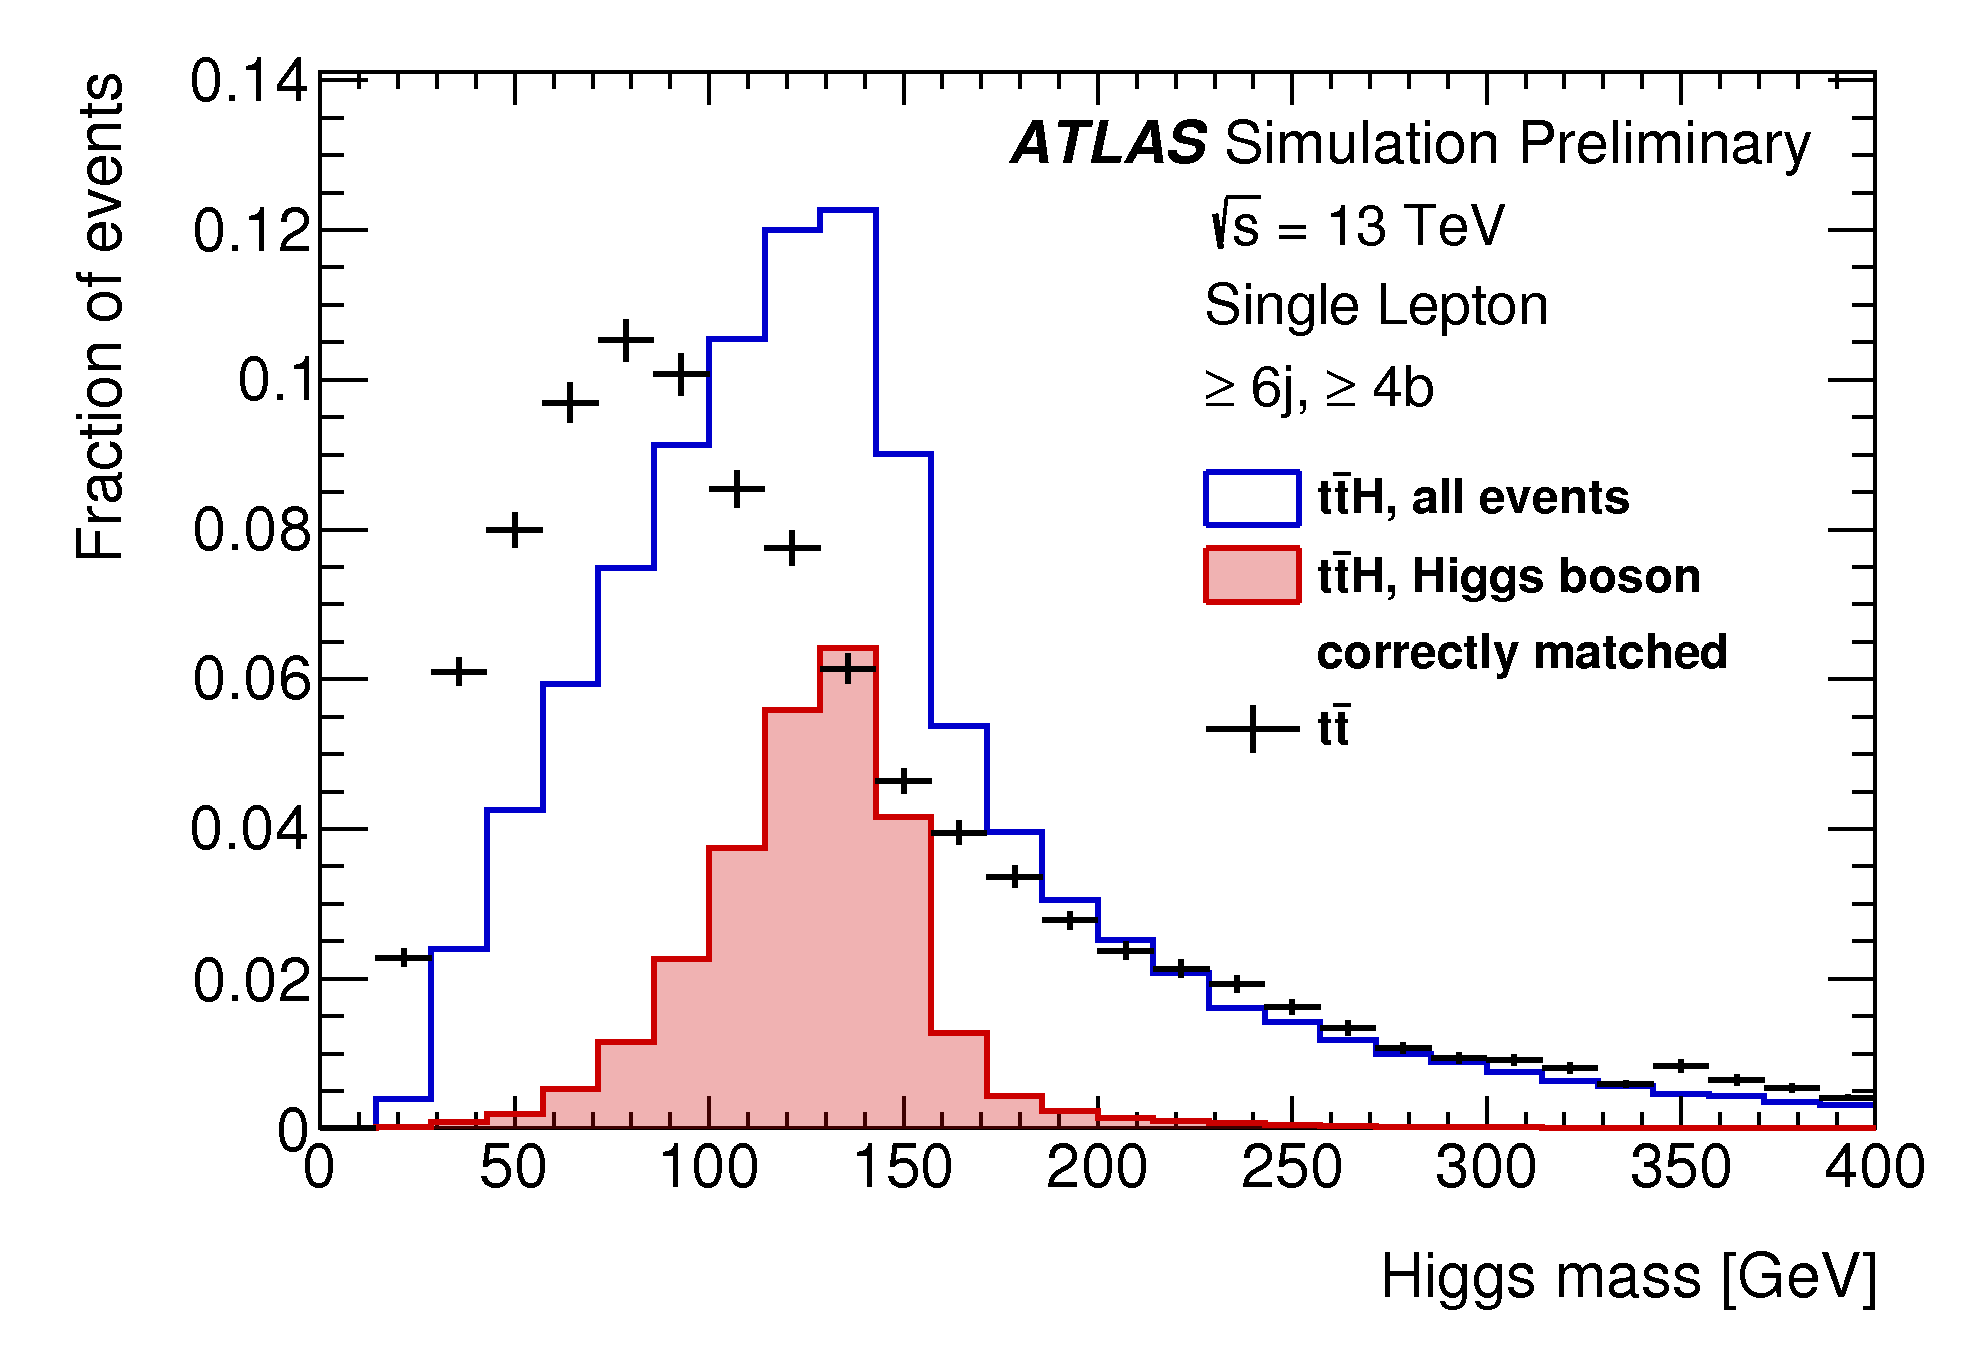
\includegraphics[width=0.5\textwidth]{figures/ttH/fig_05b.png}
\captionsetup{width=0.85\textwidth} \caption{\small The reconstructed Higgs-boson invariant mass in the ($\ge$6j, $\ge$4b) region, from the reconstruction BDT that does not use Higgs-related input variables. All signal events are shown in blue, while those with the correct jets assigned to the Higgs boson are shown in red. The $t\bar{t}$ background, consisting primarily of $t\bar{t}+\ge1b$, is shown in black.}
\label{sec:tth:fig:recobdt}
\end{figure}


Given the difficulty to increase the purity of the signal-rich regions just using kinematic reconstruction of the $t\bar{t}H$ system, the sensitivity can only to be optimised by introducing a more powerful discriminating variable. An additional BDT, referred to as ``classification'' BDT, is trained in each signal region (5j, $\ge$4b), ($\ge$6j, 3b) and ($\ge$6j, $\ge$4b) to discriminate the $t\bar{t}H$ signal from the background. Different types of variables are considered, from simple object kinematics such as jet \pt or di-jet properties, to complex event variables that make use of the full final state. As an example of the latter, the eigenvalues of the linear momentum tensor \cite{tensor} are used to construct discriminant variables such as the aplanarity of the event. Fox-Wolfram moments are used to describe the geometrical correlation among objects in the event in terms of spherical harmonics \cite{foxW}. In general, event shape variables have the advantage that they can be constructed in all topologies and are less sensitive to the loss of jets through acceptance effects. The information coming from the two reconstruction BDTs is included as well in the classification BDT. 
All variables used for the BDT training and their pairwise correlations are required to be described well by the simulation in all regions.
The following approach is used to find an optimal set of variables in each signal-rich region: the candidate input variables are ranked by their signal-to-background separation power defined as:

\be
{\rm Sep}=\frac{1}{2}\displaystyle\sum_{i}^{\rm bins}\frac{(N_{i}^{S}-N_{i}^{B})^{2}}{N_{i}^{S}+N_{i}^{B}}, 
\ee

\noindent where $N_{i}^{S}$ and $N_{i}^{B}$ are the entries in each bin of the normalised signal and background distributions, respectively.
An iterative process then removes variables with no significant improvement of discrimination between signal and background and it stops when the best 15  variables are selected in each signal region. The complete list of variables used in the classification BDTs and their definition can be found in table \ref{sec:tth:tab:SL_classifVars}.
\begin{table*}[]\footnotesize
\centering     % 1 2 3 4 5
\begin{tabular}{|l|l|c|c|c|}
\hline       
\multirow{ 2}{*}{Variable} & \multirow{ 2}{*}{Definition}  & \multicolumn{3}{c|}{Region}
\\ %\hline
\cline{3-5}
& &  $\ge6 {\rm j},\ge4 {\rm b}$ & $\ge6 {\rm j},\,3 {\rm b}$ & $ 5 {\rm j},\ge4 {\rm b}$  \\
\hline
\multicolumn{5}{|l|}{General kinematic variables} \\ 
\hline
$\Delta R_{bb}^{\rm avg}$  & Average $\Delta R$ for all $b$-tagged jet pairs     &   \checkmark    &       \checkmark       &       \checkmark          \\ [0.1cm]

\multirow{2}{*}{\ensuremath{\Delta R^{\mathrm{max} ~ p_T}_{bb}}} & $\Delta R$ between the two $b$-tagged jets with the  &  \multirow{2}{*} {\checkmark} & \multirow{2}{*} {--} & \multirow{2}{*} {--}  \\ [-0.1cm]
               & largest vector sum $\pt$   &  & &   \\ 
$\Delta\eta_{\mathrm{jj}}^{\mathrm{max}}$ & Maximum $\Delta\eta$ between any two jets & \checkmark & \checkmark & \checkmark \\ [0.1cm]
\multirow{2}{*}{$m_{bb}^{{\rm min}\Delta R}$} & Mass of the combination of the two $b$-tagged &  \multirow{2}{*} {\checkmark}  &  \multirow{2}{*} {\checkmark}  &  \multirow{2}{*}{--}   \\ [-0.1cm]
               & jets with the smallest $\Delta R$    &    &  &       \\ 
\multirow{2}{*}{$m_{jj}^{{\rm min}\Delta R}$}  & Mass of the combination of any two jets with  & \multirow{2}{*} {--} & \multirow{2}{*} {--} & \multirow{2}{*} {\checkmark} \\ [-0.1cm]
               & the smallest $\Delta R$   &   & &       \\ 
\multirow{2}{*}{$m_{bj}^{{\rm max}~\pt}$}  & Mass of the combination of a $b$-tagged jet and  &  \multirow{2}{*} {--} &  \multirow{2}{*} {\checkmark}  &  \multirow{2}{*} {--}  \\ [-0.1cm]
               & any jet with the largest vector sum $\pt$   &     &   &     \\ 
$\pt^{\rm jet5}$ & $\pt$ of the fifth leading jet    &   \checkmark    &       \checkmark       &       \checkmark      \\  
\multirow{2}{*}{$N_{bb}^{\rm Higgs30}$} & Number of $b$-jet pairs with invariant mass within  & \multirow{2}{*}\checkmark & \multirow{2}{*} {--} & \multirow{2}{*}{\checkmark} \\ [-0.1cm]
               &  30 GeV of the Higgs boson mass &       & &     \\ 
$N_{40}^{\rm jet}$   & Number of jets with $\pt\ge40$GeV &   --    &       \checkmark       &      --      \\ [0.1cm]
$H_{T}^{\rm had}$         & Scalar sum of jet $\pt$    &   --    &       \checkmark       &       \checkmark          \\ [0.1cm]
\multirow{2}{*}{$\Delta_{{\rm lep}-bb}^{{\rm min}\Delta R}$} & $\Delta R$ between the lepton and the combination & \multirow{2}{*}  {--}  &  \multirow{2}{*}  {--}  &  \multirow{2}{*}  {\checkmark}   \\ [-0.1cm]
               & of the two $b$-tagged jets with the smallest $\Delta R$   & & &    \\ 
\multirow{2}{*}{Aplanarity}    & $1.5 \lambda_2$, where $\lambda_2$ is the second eigenvalue of the   & \multirow{2}{*} {\checkmark}  & \multirow{2}{*} {\checkmark} & \multirow{2}{*} {\checkmark}  \\ [-0.1cm]
               & momentum tensor \cite{tensor} built with all jets    &   & & \\ 
\multirow{2}{*}{Centrality}   & Scalar sum of the $\pt$ divided by sum of the $E$ for & \multirow{2}{*} {\checkmark}   &  \multirow{2}{*} {\checkmark}  &  \multirow{2}{*} {\checkmark}   \\ [-0.1cm]
               & all jets and the lepton   & & &  \\
\multirow{2}{*}{$H1$}  & Second Fox--Wolfram moment computed using &  \multirow{2}{*} {\checkmark}  &  \multirow{2}{*} {\checkmark}  &  \multirow{2}{*} {\checkmark}     \\ [-0.1cm]
               & all jets and the lepton      &       &        &    \\ 
 \hline
\multicolumn{5}{|l|}{Variables from reconstruction BDT output} \\
\hline
BDT output      &                 & \checkmark$^*$ & \checkmark$^*$  & \checkmark$^*$ \\
$m_{H}$     & Higgs boson mass   & \checkmark & \checkmark  & \checkmark\\ 
$m_{H,b_{\rm lep~top}}$ & Mass of Higgs boson and $b$-jet from leptonic top  & \checkmark & --          & --\\
$\Delta R_{\rm Higgs~bb}$ & $\Delta R$ between $b$-jets from the Higgs boson  & \checkmark & \checkmark  & \checkmark\\ 
$\Delta R_{H,t\bar{t}}$ & $\Delta R$ between Higgs boson and $t\bar{t}$ system  & \checkmark$^*$ & \checkmark$^*$  & \checkmark$^*$ \\
$\Delta R_{H,{\rm lep~top}}$&  $\Delta R$ between Higgs boson and leptonic top  & \checkmark & --          & --\\
$\Delta R_{H,b_{\rm had~top}}$& $\Delta R$ between Higgs boson and $b$-jet from hadronic top      & --         & \checkmark$^*$  & \checkmark$^*$ \\
\hline
\end{tabular}
\captionsetup{width=0.85\textwidth} \caption{\small Definition of the variables used in the classification BDT for the signal regions. For the variables from the reconstruction BDT, those with a $^{*}$ are from the BDT using Higgs-boson information, while those with no $^{*}$ are from the BDT without Higgs-boson information. }
\label{sec:tth:tab:SL_classifVars}
\end{table*}
Figure \ref{sec:ttH:fig:classBDT} shows the distribution of the resulting classification BDT defined in each of the signal-rich regions.



\begin{figure}[t!]
\begin{subfigure}{0.5\textwidth}
  \centering
  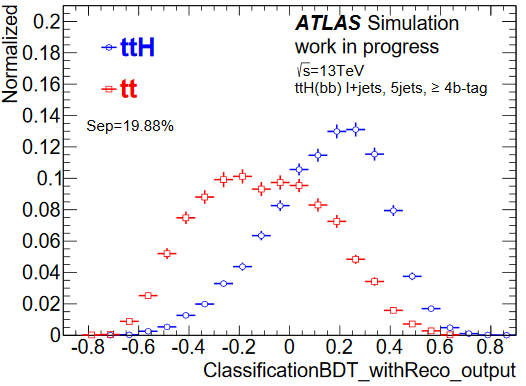
\includegraphics[width=0.9\textwidth]{figures/ttH/bdt54.png}
  \caption{}
  \label{sec:obj:fig:beff}
\end{subfigure}
\begin{subfigure}{0.5\textwidth}
  \centering
  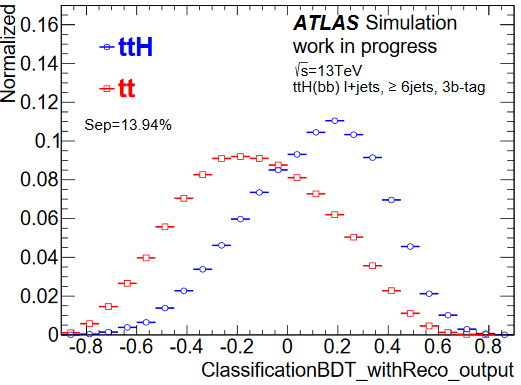
\includegraphics[width=0.9\textwidth]{figures/ttH/bdt63.png}
  \caption{}
  \label{sec:obj:fig:ceff}
\end{subfigure}
\begin{center}
\begin{subfigure}{0.5\textwidth}
  \centering
  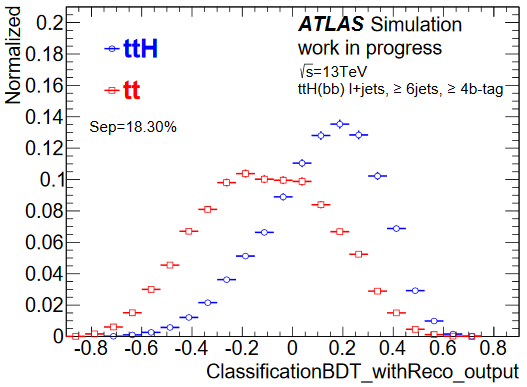
\includegraphics[width=0.9\textwidth]{figures/ttH/bdt64.png}
  \caption{}
  \label{sec:obj:fig:leff}
\end{subfigure}
\end{center}
\captionsetup{width=0.85\textwidth} \caption{\small Comparison of the shape of the classification BDT output distribution between $t\bar{t}H(H \to b\bar{b})$ signal and $t\bar{t}+$jets background in the (a) (5j, $\ge4$b), (b) ($\ge$6j, 3b) and (c) ($\ge$6j, $\ge$4b) regions.}
\label{sec:ttH:fig:classBDT}
\end{figure}
